\chapter{STR solutions}
\begin{abox}
	Practice set 1 solutions
	\end{abox}
\begin{enumerate}
\begin{minipage}{\textwidth}
	\item Consider the decay process $\tau^{-} \rightarrow \pi^{-}+v_{\tau}$ in the rest frame of the $\tau^{-} .$The masses of the $\tau^{-}, \pi^{-}$and $v_{\tau}$ are $M_{\tau}, M_{\pi}$ and zero respectively.\\
	\textbf{A} The energy of $\pi^{-}$is
	\exyear{NET JUNE 2011}
\end{minipage}
\begin{tasks}(2)
	\task[\textbf{A.}] $\frac{\left(M_{\tau}^{2}-M_{\pi}^{2}\right) c^{2}}{2 M_{\tau}}$
	\task[\textbf{B.}]$\frac{\left(M_{\tau}^{2}+M_{\pi}^{2}\right) c^{2}}{2 M_{\tau}}$
	\task[\textbf{C.}]$\left(M_{\tau}-M_{\pi}\right) c^{2}$
	\task[\textbf{D.}]$\sqrt{M_{\tau} M_{\pi}} c^{2}$
\end{tasks}
\begin{answer}
	\begin{align*}
	\text { From conservation of energy } M_{\tau} c^{2}&=E_{\pi}+E_{v} \text {. }\\
	E_{\pi}^{2}&=p^{2} c^{2}+M_{\pi}^{2} c^{4} \text { and } E_{v}^{2}=p^{2} c^{2} \text { since momentum of } \pi^{-} \text {and } v_{\tau} \text { is same. }\\
	M_{\tau} c^{2}&=E_{\pi}+E_{v}, M_{\pi}^{2} c^{4}=E_{\pi}^{2}-E_{v}^{2} \Rightarrow E_{\pi}-E_{v}=\frac{M_{\pi}^{2} c^{4}}{M_{\tau} c^{2}}\\
	E_{\pi}-E_{v}&=\frac{M_{\pi}^{2} c^{2}}{M_{\tau}} \text { and } E_{\pi}+E_{v}=M_{\tau} c^{2} \Rightarrow E_{\pi}=\frac{\left(M_{\tau}^{2}+M_{\pi}^{2}\right) c^{2}}{2 M_{\tau}}
	\end{align*}
	The correct option is \textbf{(b)}
\end{answer}
\textbf{B} The velocity of  $\pi^{-} \text {is }$
\begin{tasks}(1)
	\task[\textbf{A.}] $\frac{\left(M_{\tau}^{2}-M_{\pi}^{2}\right) c}{M_{\tau}^{2}+M_{\pi}^{2}}$
	\task[\textbf{B.}]$\frac{\left(M_{\tau}^{2}+M_{\pi}^{2}\right) c}{M_{\tau}^{2}-M_{\pi}^{2}}$ 
	\task[\textbf{C.}] $\frac{M_{\pi} c}{M_{\tau}}$
	\task[\textbf{D.}]$\frac{M_{\tau} c}{M_{\pi}}$
\end{tasks}
\begin{answer}
\begin{align*}
\text { Velocity of } \pi^{-} \quad E_{\pi}&=\frac{\left(M_{\tau}^{2}+M_{\pi}^{2}\right) c^{2}}{2 M_{\tau}}=\frac{M_{\pi} c^{2}}{\sqrt{1-\frac{v^{2}}{c^{2}}}} \Rightarrow\left(1-\frac{v^{2}}{c^{2}}\right)=\frac{4 M_{\pi}^{2} M_{\tau}^{2}}{\left(M_{\tau}^{2}+M_{\pi}^{2}\right)^{2}}\\
\Rightarrow \frac{v^{2}}{c^{2}}&=1-\frac{4 M_{\pi}^{2} M_{\tau}^{2}}{\left(M_{\tau}^{2}+M_{\pi}^{2}\right)^{2}}\\
\frac{v^{2}}{c^{2}}&=\frac{M_{\tau}^{4}+M_{\pi}^{4}+2 M_{\tau}^{2} M_{\pi}^{2}-4 M_{\pi}^{2} M_{\tau}^{2}}{\left(M_{\tau}^{2}+M_{\pi}^{2}\right)^{2}}\\
v&=\left(\frac{M_{\tau}^{2}-M_{\pi}^{2}}{M_{\tau}^{2}+M_{\pi}^{2}}\right) c
\end{align*}
The correct option is \textbf{(a)}	
\end{answer}
\begin{minipage}{\textwidth}
	\item A constant force $F$ is applied to a relativistic particle of rest mass $m$. If the particle starts from rest at $t=0$, its speed after a time $t$ is
	\exyear{NET DEC 2011}
\end{minipage}
\begin{tasks}(2)
	\task[\textbf{A.}] $\mathrm{Ft} / \mathrm{m}$
	\task[\textbf{B.}]$c \tanh \left(\frac{F t}{m c}\right)$
	\task[\textbf{C.}]$c\left(1-e^{-F t / m c}\right)$
	\task[\textbf{D.}]$\frac{F c t}{\sqrt{F^{2} t^{2}+m^{2} c^{2}}}$
\end{tasks}
\begin{answer}
	\begin{align*}
	\frac{d p}{d t}&=F \Rightarrow p=F t+c . \text { At } t=0, p=0 \text { so, } c=0\\
	p&=F t \Rightarrow \frac{m u}{\sqrt{1-\frac{u^{2}}{c^{2}}}}\\
	u&=\frac{\left(\frac{F}{m}\right) t}{\sqrt{1+\left(\frac{F t}{m c}\right)^{2}}}=\frac{F c t}{\sqrt{F^{2} t^{2}+m^{2} c^{2}}}\\
	\end{align*}
	The correct option is \textbf{(d)}
\end{answer}
\begin{minipage}{\textwidth}
	\item Two events separated by a (spatial) distance $9 \times 10^{9} \mathrm{~m}$, are simultaneous in one inertial frame. The time interval between these two events in a frame moving with a constant speed $0.8 c$ (where the speed of light $c=3 \times 10^{8} \mathrm{~m} / \mathrm{s}$ ) is
	\exyear{NET JUNE 2012}
\end{minipage}
\begin{tasks}(2)
	\task[\textbf{A.}] $60 \mathrm{~s}$
	\task[\textbf{B.}]$40 \mathrm{~s}$
	\task[\textbf{C.}]$20 s$
	\task[\textbf{D.}] $0 s$
\end{tasks}
\begin{answer}
	\begin{align*}
	x_{2}^{\prime}-x_{1}^{\prime}&=9 \times 10^{9} m \text { and } t_{2}^{\prime}-t_{1}^{\prime}=0 . \text { Then }\\
	t_{2}-t_{1}&=\left(\frac{t_{2}^{\prime}+\frac{v}{c^{2}} x_{2}^{\prime}}{\sqrt{1-\frac{v^{2}}{c^{2}}}}\right)-\left(\frac{t_{1}^{1}+\frac{v}{c^{2}} x_{1}^{\prime}}{\sqrt{1-\frac{v^{2}}{c^{2}}}}\right)\\
	t_{2}-t_{1}&=\frac{t_{2}^{\prime}-t_{1}^{\prime}}{\sqrt{1-\frac{v^{2}}{c^{2}}}}+\frac{v}{c^{2}} \frac{\left(x_{2}^{\prime}-x_{1}^{\prime}\right)}{\sqrt{1-\frac{v^{2}}{c^{2}}}}=\frac{v}{c^{2}} \frac{\left(x_{2}^{\prime}-x_{1}^{\prime}\right)}{\sqrt{1-\frac{v^{2}}{c^{2}}}}\\
	\text { Put } v&=0.8 c \quad \Rightarrow t_{2}-t_{1} \cong 40 \mathrm{sec}
	\end{align*}
	The correct option is \textbf{(b)}
\end{answer}
\begin{minipage}{\textwidth}
	\item What is proper time interval between the occurrence of two events if in one inertial frame events are separated by $7.5 \times 10^{8} \mathrm{~m}$ and occur $6.5 \mathrm{~s}$ apart?
	\exyear{NET JUNE 2012}
\end{minipage}
\begin{tasks}(2)
	\task[\textbf{A.}] $6.50 \mathrm{~s}$
	\task[\textbf{B.}]$6.00 \mathrm{~s}$
	\task[\textbf{C.}]$5.75 \mathrm{~s}$
	\task[\textbf{D.}]$5.00 \mathrm{~s}$
\end{tasks}
\begin{answer}
	\begin{align*}
	\text{Proper time interval}
	\Delta t=\sqrt{\left(\Delta t^{\prime}\right)^{2}-\frac{r^{2}}{c^{2}}}=\sqrt{(6.5)^{2}-\left(\frac{7.5}{3}\right)^{2}}=6 \text { sec. }
	\end{align*}
	The correct option is \textbf{(b)}
\end{answer}
\begin{minipage}{\textwidth}
	\item The muon has mass $105 \mathrm{MeV} / \mathrm{c}^{2}$ and mean life time $2.2 \mu \mathrm{s}$ in its rest frame. The mean distance traversed by a muon of energy $315 \mathrm{MeV}$ before decaying is approximately,
	\exyear{NET DEC 2012}
\end{minipage}
\begin{tasks}(2)
	\task[\textbf{A.}] $3 \times 10^{5} \mathrm{~km}$ 
	\task[\textbf{B.}]$2.2 \mathrm{~cm}$
	\task[\textbf{C.}]$6.6 \mu \mathrm{m}$
	\task[\textbf{D.}]$1.98 \mathrm{~km}$
\end{tasks}
\begin{answer}
	\begin{align*}
	\text { Since } E&=315 \mathrm{MeV} \text { and } m_{0}=105 \frac{\mathrm{MeV}}{c^{2}} \text {. }\\
	E=m c^{2} \Rightarrow E&=\frac{m_{0} c^{2}}{\sqrt{1-\frac{v^{2}}{c^{2}}}} \Rightarrow 315	\\
	315&=\frac{105}{\sqrt{1-\frac{v^{2}}{c^{2}}}} \Rightarrow v=0.94 c\\
	\text{Now}, t&=\frac{t_{0}}{\sqrt{1-\frac{v^{2}}{c^{2}}}}\\
	t_{0}&=2.2 \mu s \Rightarrow t=\frac{2.2 \times 10^{-6}}{\sqrt{1-\frac{8}{9}}} \Rightarrow t=6.6 \mu s\\
	\text { Now the distance traversed by muon is } v t&=0.94 c \times 6.6 \times 10^{-6}=1.86 \mathrm{~km} \text {. }
	\end{align*}
	The correct option is \textbf{(d)}
\end{answer}
\begin{minipage}{\textwidth}
	\item The area of a disc in its rest frame $S$ is equal to 1 (in some units). The disc will appear distorted to an observer $O$ moving with a speed $u$ with respect to $S$ along the plane of the disc. The area of the disc measured in the rest frame of the observer $O$ is $(c$ is the speed of light in vacuum)
	\exyear{NET JUNE 2013}
\end{minipage}
\begin{tasks}(2)
	\task[\textbf{A.}] $\left(1-\frac{u^{2}}{c^{2}}\right)^{1 / 2}$
	\task[\textbf{B.}]$\left(1-\frac{u^{2}}{c^{2}}\right)^{-1 / 2}$
	\task[\textbf{C.}]$\left(1-\frac{u^{2}}{c^{2}}\right)$
	\task[\textbf{D.}]$\left(1-\frac{u^{2}}{c^{2}}\right)^{-1}$
\end{tasks}
\begin{answer}
\begin{align*}
&\text { Area of disc from } \mathrm{S} \text { frame is } 1 \text { i.e. } \pi a^{2}=1 \text { or } \pi a \cdot a=1\\
&\text { Area of disc from } S^{\prime} \text { frame is } \pi a \cdot b=\pi a \cdot a \sqrt{1-\frac{u^{2}}{c^{2}}}=1 \cdot \sqrt{1-\frac{u^{2}}{c^{2}}}=\sqrt{1-\frac{u^{2}}{c^{2}}}\\
&\text { where } b=a \sqrt{1-\frac{u^{2}}{c^{2}}}
\end{align*}
The correct option is \textbf{(a)}	
\end{answer}
\begin{minipage}{\textwidth}
	\item The recently-discovered Higgs boson at the LHC experiment has a decay mode into a photon and a $Z$ boson. If the rest masses of the Higgs and $Z$ boson are $125 \mathrm{GeV} / \mathrm{c}^{2}$ and $90 \mathrm{GeV} / \mathrm{c}^{2}$ respectively, and the decaying Higgs particle is at rest, the energy of the photon will approximately be
	\exyear{NET JUNE 2014}
\end{minipage}
\begin{tasks}(2)
	\task[\textbf{A.}] $35 \sqrt{3} \mathrm{GeV}$
	\task[\textbf{B.}]$35 \mathrm{GeV}$
	\task[\textbf{C.}]$30 \mathrm{GeV}$
	\task[\textbf{D.}]$15 \mathrm{GeV}$
\end{tasks}
\begin{answer}
	\begin{align*}
	H_{B} &\rightarrow P_{H}+Z_{B}\\
	\intertext { From conservation of momentum }
	 0&=\vec{P}_{1}+\vec{P}_{2} \Rightarrow \vec{P}_{1}=-\vec{P}_{2} \Rightarrow\left|P_{1}\right|=\left|P_{2}\right|\\
	\text { Now } E_{H_{B}}&=E_{P_{H}}+E_{Z_{B}} \Rightarrow E_{P_{H}}+E_{Z_{B}}=M_{H_{B}} c^{2}\\
	E_{P_{H}}^{2}&=P_{1}^{2} c^{2}+0 \text { and } E_{Z_{B}}^{2}=P_{2}^{2} c^{2}+M_{Z_{B}}^{2} c^{4}\\
	&\Rightarrow\left(E_{Z_{B}}-E_{P_{H}}\right)\left(E_{Z_{B}}+E_{P_{H}}\right)=M_{Z_{B}}^{2} c^{4} \quad \because\left|P_{1}\right|=\left|P_{2}\right|\\
	&\Rightarrow E_{Z_{B}}-E_{P_{H}}=\frac{M_{Z_{B}}^{2} c^{4}}{M_{H_{B}} c^{2}}=\frac{M_{Z_{B}}^{2} c^{2}}{M_{H_{B}}} \quad \because E_{Z_{B}}+E_{P_{H}}=M_{H_{B}} c^{2}\\
	&\Rightarrow 2 E_{P_{H}}=M_{H_{B}} c^{2}-\frac{M_{z_{B}}^{2} c^{2}}{M_{H_{B}}} \Rightarrow E_{P_{H}}=\frac{\left(M_{H_{B}}^{2}-M_{z_{B}}^{2}\right) c^{2}}{M_{H_{B}}}\\
	&\Rightarrow E_{P_{H}}=\left(\frac{125 \times 125-90 \times 90}{2 \times 125}\right) \times \frac{c^{4}}{c^{4}}=30.1 \mathrm{GeV}
	\end{align*}
	The correct option is \textbf{(c)}
\end{answer}
\begin{minipage}{\textwidth}
	\item Consider three inertial frames of reference $A, B$ and $C$. the frame $B$ moves with a velocity $\frac{c}{2}$ with respect to $A$, and $C$ moves with a velocity $\frac{c}{10}$ with respect to $B$ in the same direction. The velocity of $C$ as measured in $A$ is
	\exyear{NET JUNE 2015}
\end{minipage}
\begin{tasks}(2)
	\task[\textbf{A.}] $\frac{3 c}{7}$
	\task[\textbf{B.}]$\frac{4 c}{7}$
	\task[\textbf{C.}]$\frac{c}{7}$
	\task[\textbf{D.}] $\frac{\sqrt{3} c}{7}$
\end{tasks}
\begin{answer}$\left. \right. $	\\
\begin{minipage}{0.5\textwidth}
		\begin{align*}
	v&=\frac{c}{2}, \quad u_{x}^{\prime}=\frac{c}{10}\\
	u_{x}&=\frac{u_{x}^{\prime}+v}{1+\frac{u^{\prime} v_{x}}{c^{2}}}=\frac{4 c}{7}
	\end{align*}
\end{minipage}
	\begin{minipage}{0.5\textwidth}
	\begin{figure}[H]
		\centering
		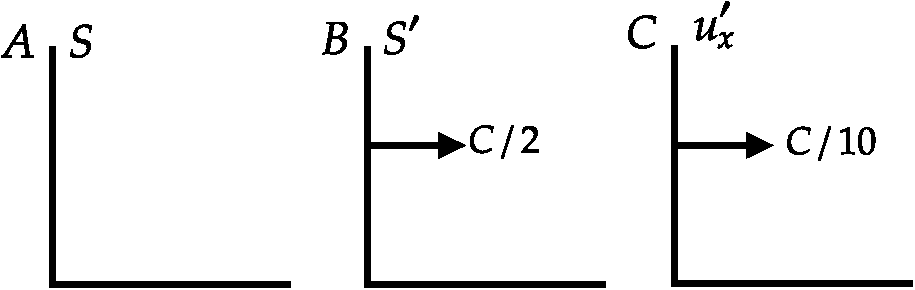
\includegraphics[height=3cm,width=5cm]{NET 1}
	\end{figure}
	\end{minipage}
The correct option is \textbf{(b)}
\end{answer}
\begin{minipage}{\textwidth}
	\item Consider a particle of mass $m$ moving with a speed $v$. If $T_{R}$ denotes the relativistic kinetic energy and $T_{N}$ its non-relativistic approximation, then the value of $\frac{\left(T_{R}-T_{N}\right)}{T_{R}}$ for $v=0.01 c$, is
	\exyear{NET DEC 2015}
\end{minipage}
\begin{tasks}(2)
	\task[\textbf{A.}] $1.25 \times 10^{-5}$
	\task[\textbf{B.}]$5.0 \times 10^{-5}$
	\task[\textbf{C.}]$7.5 \times 10^{-5}$
	\task[\textbf{D.}]$1.0 \times 10^{-4}$
\end{tasks}
\begin{answer}
	\begin{align*}
	T_{N}&=\frac{1}{2} m_{0} v^{2}, T_{R}=m c^{2}-m_{0} c^{2}=\frac{m_{0} c^{2}}{\sqrt{1-\frac{v^{2}}{c^{2}}}}-m_{0} c^{2} \quad(\because v=0.01 c)\\
	\text { Now, } \frac{\left(T_{R}-T_{N}\right)}{T_{R}}&=1-\frac{T_{N}}{T_{R}}=1-\frac{\frac{1}{2} m_{0} v^{2}}{\frac{m_{0} c^{2}}{\sqrt{1-\frac{v^{2}}{c^{2}}}}-m_{0} c^{2}}\\
	&=1-\frac{\frac{\frac{v^{2}}{2}}{c^{2}}}{\sqrt{1-\frac{v^{2}}{c^{2}}}-c^{2}}=1-\frac{\frac{(0.01)^{2}}{2}}{\frac{1}{\sqrt{1-(0.01)^{2}}}}-1\\
	\frac{T_{R}-T_{N}}{T_{R}}&=0.75
	\end{align*}
	None of the option is correct.
\end{answer}
\begin{minipage}{\textwidth}
	\item Let $(x, t)$ and $\left(x^{\prime}, t^{\prime}\right)$ be the coordinate systems used by the observers $O$ and $O^{\prime}$, respectively. Observer $O^{\prime}$ moves with a velocity $v=\beta c$ along their common positive $x$ axis. If $x_{+}=x+c t$ and $x_{-}=x-c t$ are the linear combinations of the coordinates, the Lorentz transformation relating $O$ and $O^{\prime}$ takes the form
	\exyear{NET JUNE 2016}
\end{minipage}
\begin{tasks}(2)
	\task[\textbf{A.}] $x_{+}^{\prime}=\frac{x_{-}-\beta x_{+}}{\sqrt{1-\beta^{2}}}$ and $x_{-}^{\prime}=\frac{x_{+}-\beta x_{-}}{\sqrt{1-\beta^{2}}}$
	\task[\textbf{B.}]$x_{+}^{\prime}=\sqrt{\frac{1+\beta}{1-\beta}} x_{+}$and $x_{-}^{\prime}=\sqrt{\frac{1-\beta}{1+\beta}} x_{-}$
	\task[\textbf{C.}]$x_{+}^{\prime}=\frac{x_{+}-\beta x_{-}}{\sqrt{1-\beta^{2}}}$ and $x_{-}^{\prime}=\frac{x_{-}-\beta x_{+}}{\sqrt{1-\beta^{2}}}$
	\task[\textbf{D.}]$x_{+}^{\prime}=\sqrt{\frac{1-\beta}{1+\beta}} x_{+}$and $x_{-}^{\prime}=\sqrt{\frac{1+\beta}{1-\beta}} x_{-}$
\end{tasks}
\begin{answer}
\begin{align*}
x_{+}^{\prime}&=x^{\prime}+c t^{\prime}\\
&=\frac{x-v t}{\sqrt{1-\frac{v^{2}}{c^{2}}}}+\frac{c\left(t-\frac{v x}{c^{2}}\right)}{\sqrt{1-\frac{v^{2}}{c^{2}}}}=\frac{x\left(1-\frac{v}{c}\right)}{\sqrt{1-\frac{v^{2}}{c^{2}}}}+\frac{c t\left(1-\frac{v}{c}\right)}{\sqrt{1-\frac{v^{2}}{c^{2}}}}\\
&=x \sqrt{\frac{1-\frac{v}{c}}{1+\frac{v}{c}}}+c t \sqrt{\frac{1-\frac{v}{c}}{1+\frac{v}{c}}}=\sqrt{\frac{1-\frac{v}{c}}{1+\frac{v}{c}}}(x+c t)\\
x_{+}^{\prime}&=\sqrt{\frac{1-\beta}{1+\beta}} x_{+}\\
x_{-}^{\prime}&=x^{\prime}-c t^{\prime}=\frac{x-v t}{\sqrt{1-\frac{v^{2}}{c^{2}}}}-\frac{c\left(t-\frac{v x}{c^{2}}\right)}{\sqrt{1-\frac{v^{2}}{c^{2}}}}=\frac{x\left(1+\frac{v}{c}\right)}{\sqrt{1-\frac{v^{2}}{c^{2}}}}-\frac{c t\left(1+\frac{v}{c}\right)}{\sqrt{1-\frac{v^{2}}{c^{2}}}}\\
x_{-}^{\prime}&=x \sqrt{\frac{1+\frac{v}{c}}{1-\frac{v}{c}}}-c t \sqrt{\frac{1+\frac{v}{c}}{1-\frac{v}{c}}} \Rightarrow x_{-}^{\prime}=\sqrt{\frac{1+\beta}{1-\beta}}(x-c t) \Rightarrow x_{-}^{\prime}=\sqrt{\frac{1+\beta}{1-\beta} x_{-}}
\end{align*}
The correct option is \textbf{(d)}	
\end{answer}
\begin{minipage}{\textwidth}
	\item For a particle of energy $E$ and momentum $p$ (in a frame $F$ ), the rapidity $y$ is defined as $y=\frac{1}{2} \ln \left(\frac{E+p_{3} c}{E-p_{3} c}\right) .$ In a frame $F^{\prime}$ moving with velocity $v=(0,0, \beta c)$ with respect to $F$, the rapidity $y^{\prime}$ will be
	\exyear{NET JUNE 2016}
\end{minipage}
\begin{tasks}(2)
	\task[\textbf{A.}] $y^{\prime}=y+\frac{1}{2} \ln \left(1-\beta^{2}\right)$
	\task[\textbf{B.}]$y^{\prime}=y-\frac{1}{2} \ln \left(\frac{1+\beta}{1-\beta}\right)$
	\task[\textbf{C.}]$y^{\prime}=y+\ln \left(\frac{1+\beta}{1-\beta}\right)$
	\task[\textbf{D.}]$y^{\prime}=y+2 \ln \left(\frac{1+\beta}{1-\beta}\right)$
\end{tasks}
\begin{answer}
\begin{align*}
y&=\frac{1}{2} \ln \left(\frac{E+p_{3} c}{E-p_{3} c}\right)\\
\text { Then } y^{\prime}&=\frac{1}{2} \ln \left(\frac{E^{\prime}+p_{3}^{\prime} c}{E^{\prime}-p_{3}^{\prime} c}\right)\\
\text { Where } p_{3}^{\prime}&=\gamma\left(p_{3}-v\left(\frac{E}{c^{2}}\right)\right) \quad E^{\prime}=\gamma\left(E-v p_{3}\right)\\
\text { Put the value of } p_{3}^{\prime} \text { and } E^{\prime} \text { one will get } y^{\prime}&=\frac{1}{2} \ln \left(\frac{\left(E+p_{3} c\right)-\frac{v}{c}\left(E+p_{3} c\right)}{\left(E-p_{3} c\right)+\frac{v}{c}\left(E-p_{3} c\right)}\right)\\
\frac{1}{2} \ln \left(\frac{\left(E+p_{3} c\right)(1-\beta)}{\left(E-p_{3} c\right)(1+\beta)}\right) &\Rightarrow \frac{1}{2} \ln \left(\frac{\left(E+p_{3} c\right)}{\left(E-p_{3} c\right)}\right)+\frac{1}{2} \ln \left(\frac{1-\beta}{1+\beta}\right)\\
y+\frac{1}{2} \ln \left(\frac{1-\beta}{1+\beta}\right)& \Rightarrow y-\frac{1}{2} \ln \left(\frac{1+\beta}{1-\beta}\right)
\end{align*}
The correct option is \textbf{(b)}	
\end{answer}
\begin{minipage}{\textwidth}
	\item A relativistic particle moves with a constant velocity $v$ with respect to the laboratory frame. In time $\tau$, measured in the rest frame of the particle, the distance that it travels in the laboratory frame is
	\exyear{NET DEC 2016}
\end{minipage}
\begin{tasks}(2)
	\task[\textbf{A.}] $v \tau$
	\task[\textbf{B.}]$\frac{c \tau}{\sqrt{1-\frac{v^{2}}{c^{2}}}}$
	\task[\textbf{C.}]$v \tau \sqrt{1-\frac{v^{2}}{c^{2}}}$
	\task[\textbf{D.}]$\frac{v \tau}{\sqrt{1-\frac{v^{2}}{c^{2}}}}$
\end{tasks}
\begin{answer}$\left. \right. $\\
	\begin{minipage}{0.5\textwidth}
	\begin{align*}
	\text { From Particle } x_{1}^{\prime}&=0 x_{2}^{\prime}=0\\
	t_{\text {initial }}&=t_{1}^{\prime} \quad t_{\text {final }}=t_{2}^{\prime}\\
	x_{1}&=\frac{x_{1}^{\prime}+v t_{1}^{\prime}}{\sqrt{1-v^{2} / c^{2}}}, x_{2}=\frac{x_{2}^{\prime}+v t_{2}^{\prime}}{\sqrt{1-v^{2} / c^{2}}}\\
	x_{2}-x_{1}&=\frac{x_{2}^{\prime}-x_{1}^{\prime}}{\sqrt{1-v^{2} / c^{2}}}+\frac{v\left(t_{2}^{\prime}-t_{1}^{\prime}\right)}{\sqrt{1-v^{2} / c^{2}}}\\
	\Delta x&=\frac{v\left(t_{2}^{\prime}-t_{1}^{\prime}\right)}{\sqrt{1-v^{2} / c^{2}}}=\frac{v \tau}{\sqrt{1-v^{2} / c^{2}}}
	\end{align*}	
	\end{minipage}
\begin{minipage}{0.5\textwidth}
	\begin{figure}[H]
		\centering
		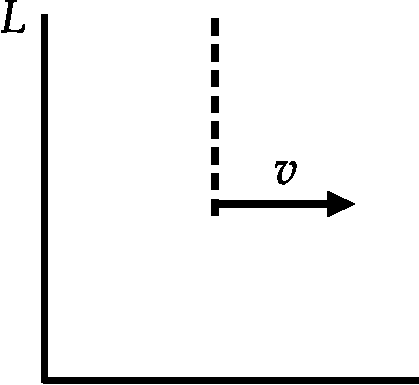
\includegraphics[height=3cm,width=5cm]{problem 2}
	\end{figure}
\end{minipage}
The correct option is \textbf{(d)}
\end{answer}
\begin{minipage}{\textwidth}
	\item Consider a radioactive nucleus that is travelling at a speed $\frac{c}{2}$ with respect to the lab frame. It emits $\gamma$-rays of frequency $v_{0}$ in its rest frame. There is a stationary detector, (which is not on the path of the nucleus) in the lab. If a $\gamma$-ray photon is emitted when the nucleus is closest to the detector, its observed frequency at the detector is
	\exyear{NET DEC 2016}
\end{minipage}
\begin{tasks}(2)
	\task[\textbf{A.}] $\frac{\sqrt{3}}{2} v_{0}$
	\task[\textbf{B.}]$\frac{1}{\sqrt{3}} v_{0}$
	\task[\textbf{C.}]$\frac{1}{\sqrt{2}} v_{0}$
	\task[\textbf{D.}]$\sqrt{\frac{2}{3}} v_{0}$
\end{tasks}
\begin{answer}
	\begin{align*}
	v&=v_{0} \sqrt{1-\frac{v^{2}}{c^{2}}} \quad \text { (If detector is not in the path at nucleus) }\\
	v&=v_{0} \sqrt{1-\frac{1}{4}}=v_{0} \frac{\sqrt{3}}{2}
	\end{align*}
	The correct option is \textbf{(a)}
\end{answer}
\begin{minipage}{\textwidth}
	\item An inertial observer sees two events $E_{1}$ and $E_{2}$ happening at the same location but $6 \mu s$ apart in time. Another observer moving with a constant velocity $v$ (with respect to the first one) sees the same events to be $9 \mu s$ apart. The spatial distance between the events, as measured by the second observer, is approximately
	\exyear{NET JUNE 2017}
\end{minipage}
\begin{tasks}(2)
	\task[\textbf{A.}] $300 m$
	\task[\textbf{B.}]$1000 m$
	\task[\textbf{C.}]$2000 m$
	\task[\textbf{D.}]$2700 m$
\end{tasks}
\begin{answer}
\begin{align*}
	x_{2}^{1}-x_{1}^{1}&=0, t_{2}^{1}-t_{1}^{1}=6 \times 10^{-6}, t_{2}-t_{1}=9 \times 10^{-6}, x_{2}-x_{1}=?\\
t_{2}-t_{2}&=9 \times 10^{-6}\\
\left(\frac{t_{2}^{1}+\frac{v}{c^{2}} x_{2}^{1}}{\sqrt{1-v^{2} / c^{2}}}\right)-\frac{\left(t_{1}^{\prime}+\frac{v}{c^{2}} x_{1}^{\prime}\right)}{\sqrt{1-v^{2} / c^{2}}}&=9 \times 10^{-6}\\
\frac{t_{2}^{\prime}-t_{1}^{\prime}}{\sqrt{1-v^{2} / c^{2}}}&=9 \times 10^{-6} \Rightarrow \frac{6 \times 10^{-6}}{\sqrt{1-v^{2} / c^{2}}}=9 \times 10^{-6}\\
v&=\sqrt{\frac{5}{9}} c \Rightarrow \sqrt{1-\frac{v^{2}}{c^{2}}}=2 / 3\\
\left(x_{2}-x_{1}\right)&=\left(\frac{x_{2}^{\prime}+v t_{2}^{\prime}}{\sqrt{1-v^{2} / c^{2}}}\right)-\left(\frac{x_{1}^{\prime}+v t_{1}^{\prime}}{\sqrt{1-v^{2} / c^{2}}}\right)\\
\frac{v}{\sqrt{1-v^{2} / c^{2}}}\left(t_{2}^{\prime}-t_{1}^{\prime}\right)\\
\left(x_{2}-x_{1}\right)&=\frac{\sqrt{5}}{3} c \times \frac{9}{6} \times\left(6 \times 10^{-6}\right)=\frac{\sqrt{5}}{3} \times 3 \times 10^{8} \times \frac{9}{6} \times 6 \times 10^{-6}\\
&=9 \times \sqrt{5} \times 10^{2}=20.12 \times 10^{2} \simeq 2000 m
\end{align*}
The correct option is \textbf{(c)}
\end{answer}
\end{enumerate}